%------------------------------%
\selectlanguage{english}
\chapter{Abstraction-oriented resource awareness}
\label{chap:abstractions_and_resource_management}
\markboth{Abstraction-oriented resource awareness}{Chapter2}
%------------------------------%

\coolphrase {Where is the `any' key?}{Homer Simpson, in response to the message, ``Press any key''}

Defining and using software abstractions (such as classes, components and languages) are common operations when building applications.
Sometimes, it is useful to consider the problem of how instances of an abstraction consume computation resources.
For instance, computing the CPU consumed by all \textit{threads} running on a system is quite helpful for system administration purposes.
Another example is the necessity of knowing the number of instances of a given class when we are profiling applications.

As shown in the previous chapter, supporting resource management is a complex task that highly depends on the technology a system is running atop of.
In this chapter, we show that specific features of the software abstraction, which is being targeted, also influence the way resource management support is implemented.
%In this chapter we show that this support also depends on features of the software abstraction we are dealing with.
%In this chapter we show how the support that we can provide and its implementation are also driven by the specific features of the software abstraction.
Due to all these specific concerns there is considerable variability to consider when writing resource management tools; dealing with this variability is complex.

%This chapter mainly discusses how to ease the task of supporting resource-aware programming by taking into account the existence of many software abstractions.

This chapter mainly discusses how the usage of software abstractions poses new challenges when we are implementing support for resource consumption monitoring and reservation.
In particular, this chapter describes two abstractions frequently used on top of MRTEs: components (Section \ref{sec:components-oriented-resource-awareness}), and domain-specific languages (DSLs) (Section \ref{sec:DSL-on-MRTEs}).
Comprehensive discussions on how these abstractions consume resources are presented.
Moreover, state of the art approaches, for handling features specific to each abstraction, are presented and their limitations discussed.
%We tackle (Section \ref{sec:component-leverage}) the issue of how to leverage component-based architectures - to reduce the overhead of dealing with resources - by specializing resource management techniques.
%Second, since new abstractions are constantly created nowadays, having generic and efficient mechanisms for controlling how they use resources may simplify the process of providing resource awareness support.
We then present the state of the art on supporting resource consumption accounting for arbitrary abstractions (Section \ref{sec:resource-awareness-for-dsl}).

\section{Developer's View versus Tooling's View} \label{sec:chapter2-introduction}

As mentioned, building abstractions is at the core of software development.
They are meant to tackle a large number of problems in software engineering, ranging from providing better representation of the business logic to supporting application's extensibility.
Interestingly, abstractions are not built from scratch; instead, they are implemented upon other abstractions provided by the runtime environment.
This leads to the well-known layered architecture where complex features are created using more simple concepts.
In the field of operating systems, processes are built relying on low-level concepts such as hardware interrupts, context-switch, and MMU hardware.
In the area of programming languages, recursive routines are implemented upon basic hardware stack manipulation.

Once a new abstraction is implemented and its invariants defined, you can use it without a complete understanding of the implementation details.
This has profound implications in the software development process; it now requires special tooling support because developers immediately start thinking in terms of such an abstraction.
For instance, showing plain assembler instructions while debugging applications is no longer good choice once you start coding your applications in a language that includes high-level concepts such as routines, loops, and conditional-statements.
In the same way, when a profiler is used to check the memory consumption of Java-based applications, the data produced is expected to reflect terms such as \textit{object} and \textit{class}.
Ideally, tools such as editors, debuggers, and profilers must be modified to make them aware of each new abstraction introduced in the development cycle.
Likewise, mechanisms to monitor resource consumption at runtime should also be modified.
Unfortunately, this is not always the case.
For instance, often developers lack the proper tools when they implement applications that execute in MRTEs.
A couple of illustrative examples are given below; the first is related to OSGi bundles, the second to Domain-Specific Languages (DSLs).

In OSGi, bundles are deployed on top of a single JVM instance.
Due to the communication mechanism used in OSGi, where objects are routinely shared, it is complex to decide which bundle should be accounted for the consumption of a particular object.
A possible approach is deciding that an object $O$ is being consumed by a bundle if $O$'s class was loaded using the classloader $C$ associated with such a bundle.
Then, we can use this mechanism to monitor per-bundle memory consumption. 
However, a profiler must perform considerable amount of processing to collect such kind of data because it is not straightforwardly available in the JVM. 
%Since we know how to represent a bundle using Java concepts, this solution is feasible.
Given the widespread usage of OSGi, memory profilers often support collecting data regarding per-bundle memory usage.
Unfortunately, similar abstractions (components models), equally implemented atop of Java, are often not properly supported by such tools because they are not as popular as OSGi.
Hence, data must be manually aggregated when an application uses abstractions that are not supported by profilers; this is a considerable burden for developers.

The example of OSGi is also useful to highlight how some abstractions have specific requirements regarding resource consumption monitoring and reservation.
In the particular case of determining how many resources are being consumed by a bundle, it is noteworthy that there exist two ways of doing so when a bundle requests a service from another bundle.
Both approaches have pros and cons \cite{Miettinen2008,Maurel:2012:AME:2304736.2304763}.
In a first option, all resources used to satisfy a request are charged to the bundle that originally issued the request, no matter whether part of the computation is performed in other bundles.
In a second option, a bundle only consumes resources when it is executing its own code.
The important point is that, above the concern we present in the previous chapter regarding the mechanisms to support resource-aware programming, engineers also have to focus on features specific to each abstraction.

Many of the newly designed DSLs are built on top of existing object-oriented languages runtime such as the JVM. 
Therefore, people in charge of optimizing, debugging and maintaining software applications can use the existing debugger and profilers of these platforms. 
However, there is a clear mismatch between classical profilers used in object-oriented systems and the newly designed languages. 
Indeed, the concepts introduced in these new DSLs may not exhibit a straightforward mapping to the underlying object-oriented system.
As a consequence, it may be time consuming and complex to use a classical profiler to check applications that are based on these new languages.

For instance, active annotations allow developers to participate in the translation process of Xtend source code to Java code via library.
Such mechanism is often used directly by developers to introduce their own abstraction or defining their own internal DSL.
In the K3-AL\footnote{Available at https://github.com/diverse-project/k3/wiki} project, active annotations are used to create an open-class mechanism on top of Java \cite{Clifton:2000:MMO:353171.353181}. 
As a result, the annotation processor changes the program structure to implement this feature. 
It adds some methods indirection (to $AASpect$), create new set of objects that represents the state of one conceptual object ($AASpectProperty$), use the Xtend extension method feature, etc.
Figure~\ref{fig:k3-diagram} shows the result of this translation process. 
The left part illustrates the code written by the developer, the middle part shows the developer view (the code that can be written to use the open-class mechanism), the right part describes the runtime view.
In this case, an instance of an open-class is not represented by a single JVM object; instead, it is represented by scattered objects.  

\begin{figure*}
\centering
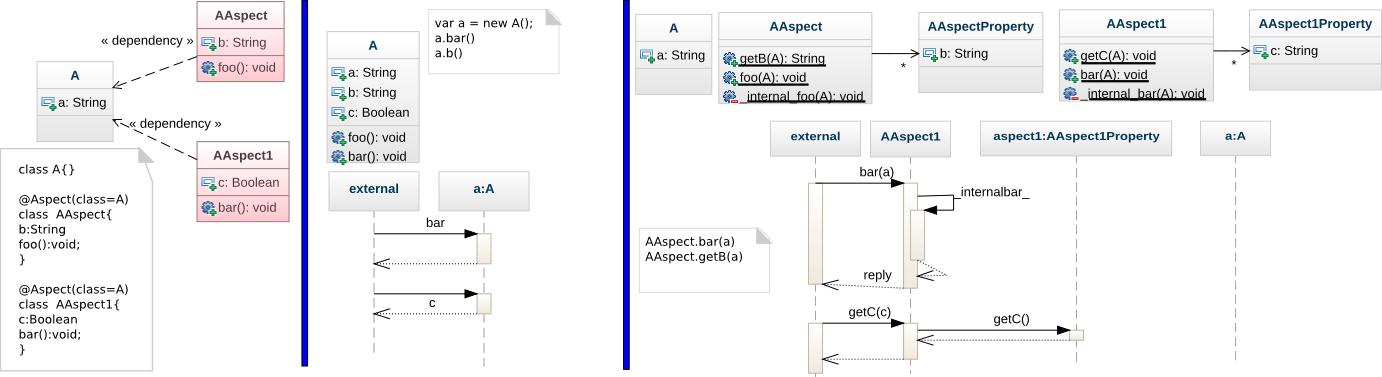
\includegraphics[width=0.9\linewidth]{chapter2/fig/famous}
\caption{Translation process used for building developer abstraction using annotations}
\label{fig:k3-diagram}
\end{figure*}

In this thesis we argue that a \textit{mismatch}, between the developer's view and the tooling's view, exists when the concepts managed by the developers are not clearly reflected in the tools.
This mismatch may complicate the development of applications, as well as prevent the correctness of software systems.
We identify in this thesis, two ways in which such a mismatch might affect software development when new software abstractions are heavily used while, at the same time, support for resource-aware programming is also required:

%\todo{This two points are really close, bad}
\begin{itemize}
\item Abstractions pose new challenges because they may have specific requirements that are not addressed by generic tools that deal with resource management.
In this case, the problem is how to reuse generic mechanisms to handle specific requirements.

\item Since new software abstractions are constantly being defined, there is an increasing pressure to ease the creation of abstraction-specific tooling support.
Simplifying the definition of tools in order to support new abstractions is the issue in this case. 
\end{itemize}

In the rest of this chapter, we extensively discuss both concerns.

\section{Specific requirements of software abstractions}
As mentioned in the previous section, when a new abstraction is defined, there is a gap between the capabilities of existent tools and users' expectations.
Therefore, it is necessary to reduce this gap by modifying generic tools to make them capable of dealing with specific features of new abstractions.

In this section, we present two kind of abstractions: software components and domain-specific languages.
The presentation aims at highlighting the type of modifications that might be required in order to make an existent approach capable of dealing with these abstractions.
Likewise, the section discuss the characteristics of components and DSLs that difficult the development of resource-aware programming tools.

To guide the discussion, the following elements are given for each type of abstraction:
\begin{itemize}
\item \textit{Introduction to the abstraction.} A brief description of the main elements of the abstraction is presented. This is focused on those features that impact resource management. 

\item \textit{Implementations of the abstraction in MRTEs.}
Illustrative cases that show how the abstraction have been implemented on top of MRTEs are described.
For instance, it briefly mentions components models that support Java.

\item An analysis of how \textit{resources are consumed} in this type of abstraction is presented.
Interestingly, there are elements that vary in the way components and DSLs consume resources.

\item \textit{Specific features to consider.}
This point makes reference to those special characteristics of the abstraction to take into account when support for resource-aware programming is implemented.     

\item \textit{Example of differences among concrete abstractions.}
Since there are, for example, many DSLs, this point aims at analysis difference among them.
In this way, we show the high degree of variability that might complicate the development of resource-aware solutions.
Instead of providing an exhaustive list of differences, we only show an illustrative one.

\item The \textit{state of the art} on providing support for resource consumption accounting and reservation for each abstraction is presented.
This is done in the form summarized discussion of existent approaches. 
\end{itemize}

This section ends by analyzing the limitation in the state of the art of both resource management for software components and DSLs. 

\subsection{Resource use in software components} \label{sec:components-oriented-resource-awareness}

Component-Based Software Engineer (CBSE) aims at developing applications by reusing independent units of software \cite{cbse-conference, Crnkovic2011}.
Through the utilization of components, connectors and configurations, CBSE reduces the complexity in the development and maintenance of systems \cite{xadl,Medvidovic:2000,VanOmmering-et-al-00}.
%In addition to economical benefits such as reducing time to market and development cost \cite{SZYPERSKI2002}, there are also technical advantages in using CBSE. 
One of its technical advantages is that it facilitates the management of dynamic architectures
~\cite{DBLP:journals/ase/NittoGMPP08, Johnson:2015:CSM:2735960.2735979}
because it simplify the implementation of features, such as, self-organizing the structure of a system, and self-adapting its behavior
\cite{PanzicaLaManna:2012:LDU:2304736.2304764, Johnson:2015:CSM:2735960.2735979,Zhang:2009:MVD:1509239.1509262}.
Likewise, many works~\cite{cbse-conference} have shown the benefits of using component-based approaches in open-world environments~\cite{baresi2006toward, Caporuscio:2010:AIA:1985522.1985547, Perez-Palacin:2010:PAO:1712605.1712614}.

Plenty of diversity exists in current component models and frameworks \cite{Heineman2001, SZYPERSKI2002, Crnkovic2011}.
They tend to target different technologies, aim at different use cases, provide support for different concerns, and use different design principles.
Crnkovic et al. \cite{Crnkovic2011} propose properties that can be used to classify component models; we are interested in those models that have the following properties:

\begin{description}
\item[Modeling capabilities:] it is common to provide a mechanism for modeling the system architecture during the development phase; this results useful to reason about the system.
In addition, it is possible to support some form of reflection for querying the architecture of a system at runtime.
Component models, which include both features, are the target of our research.

\item[Deployment of components at runtime:] since, we are dealing with the problem of supporting resource awareness in open environments, we focus on component models that allow component deployment at runtime.
Many component models are able to cope with the necessity of adaptation through, for example, the deployment of new modules, the instantiation of new services, and the creation of new bindings between components~\cite{Porter:2014:RMC:2602458.2602471, Zheng:2014:RCC:2679601.2680405, Irmert:2008:RAS:1370018.1370036, Ghezzi:2010:QDD:2163764.2163774}.
\end{description}

Other properties worth mentioning in this thesis are those that describe how components communicate.
For instance:  whether the concept of \textit{port} is implemented; if there exists distinction between \textit{required/provided interfaces}; how is the \textit{interface language}; what is the \textit{interface levels} (syntactic, semantic, behavior); and what is the \textit{communication type} (synchronous, unicast, and others).
Our interest in these properties is limited to understand what mechanisms are used to support interaction between components, how are these mechanisms implemented, and how the interaction between components affects the way in which we deal with resource consumption monitoring and reservation.

\paragraph{Usage in MRTEs}
An important property of component models is its implementation support.
The discussion in this research is limited to those that have been implemented for MRTEs.
Several component models that provide support for MRTEs have been proposed by both the industry and the academy.
Among others, we can mention Enterprise Java Beans (EJB) \cite{OracleEJB3.0}, the Open Services Gateway Initiative (OSGi) \cite{OSGI:r5}, 
Fractal \cite{Bruneton:2006:FCM:1152333.1152345}, 
SOFA 2.0 (Software Appliances) \cite{Bures2006}, Palladio \cite{}, and Kevoree~\cite{morin09a,leger2010reliable}.
It is interesting how these component models have different properties when it comes to \textit{modeling capabilities}, \textit{architecture of the system supported}, and \textit{constructs for interaction among components}.
However, they also differ in how components are represented on top of MRTE concepts; in other words, they follow different approaches to implement the component framework itself.

\paragraph{Resource consumption}

Since the lack of computational resources can break an application as easily as a violation of a business rule, dealing with resource utilization is considered an extra-function requirement~\cite{}.
Interestingly, components provide boundaries between different software entities, which are forced to communicate through well defined interfaces; it is then possible to write QoS contracts associated to these interfaces \cite{Beugnard774917}.

It is important to remember the difference between component type and component instance when we discuss the resource usage of these systems.
Indeed, instances may have a state while component types are stateless.
The distinction is important because all instances of a single component type share the same implementation.
As a consequence, it is not simple to define how a component consumes resources.
For example, the memory consumed by an instance includes those \textit{objects} used for the component framework to represent the instance itself, its ports, and bindings; it also includes the state of the component. 
However, it cannot include the memory used to store the component's code since it is shared among many instances.
Monitoring CPU and network consumption is even harder, because the code responsible for the consumption is shared.
To solve this problem, a context is associated with each component in order to determine at runtime the instance responsible of the execution of a given operation that is using resources.
Curiously, the nature of this context depends on the component model.     

\paragraph{Specific features to consider when resource awareness support is implemented}

A first issue to take into consideration is \textit{how to account for resource consumption in the presence of interaction between components}.
Usually, components are organized as clients and providers, where a component (provider) performs operations on behalf of another component (client).
It is then possible to account for resource consumption in two ways \cite{Miettinen2008,Maurel:2012:AME:2304736.2304763}:

\begin{description}
\item[direct accounting:] the resources consumed during
interaction are accounted to the provider.
For instance, the CPU used by a code that belongs
to component A is accounted to A, no matter if the code is executed on behalf of a client.

\item[indirect accounting:] all the resources consumed to serve a request that was originated in a component A are accounted to A.
In other words, there is no resource consumption accounted to service providers.
\end{description}

Both ways have advantages and disadvantages.
In the case of direct accounting, if a provider is
called in an endless loop, the resource usage will be accounted
to the provider instead of to the client that executes such a loop.
On the contrary, if a service is poorly implemented, in indirect accounting the user of the service is identified as the responsible.

A second aspect is to decide \textit{where should be implemented} the mechanism for resource consumption monitoring and reservation.
Essentially, this consists in, selecting which actors implement the mechanism and policies to manage resources, and deciding if the actors collaborate to achieve their goal \cite{Crnkovic2011}.

Many component models provide no facilities for managing extra-functional properties (EFPs) such as resource usage.
The mechanism used to handle a property is left to the designers of each application.
This facilitates the creation of EFP management policies that are tuned towards a system, but can harm the portability of components because the policies are implemented by them.

In another approach, components only address functional aspects.
Thus, in the execution environment, components
are wrapped in containers that know how to manage EFPs.
Containers can either be totally in charge of non-functional aspects or
they can interact with the component framework to manage EFPs.
This eases the inclusion of components in multiple systems where different policies for EFPs are used.

\paragraph{Example of differences among concrete abstractions}

An interesting difference that impact the implementation of mechanisms for resource consumption monitoring is how Kevoree and OSGi support interaction between components.
In Kevoree, components communicate with each other through ports.
It is straightforward to identify in the code when a component is requesting a service because a single interface (port) is used to do so, no matter if a component is using different ports. 
As a consequence, an automated tool can easily instrument the code to detect when components are communicating.
On the contrary, OSGi uses plain Java interfaces and objects to connect bundles.
In that cases it is more complex to detect when components are communicating because a bundle can communicate with several services using different interfaces. 

\paragraph{State of the art on providing resource awareness support for component-based systems}

Many works address the issue of supporting resource consumption monitoring in component-based systems.
In addition, some existent approaches present solutions for the isolation of resource consumption among components running on top of a single MRTE instance.
Unfortunately, most approaches are limited to a specific component model; in particular, a amount of work exist to solve the problem for both EJB and OSGi.

\textit{EJBMemProf}, a memory profiling framework for EJB is presented in \cite{Meyerhoefer2005}.
The main idea is executing an event handler each time a new object is created; such a handler is responsible of identifying the bundle that allocated the object.
A set of rules that guide this identification process is discussed and their accuracy evaluated.
Since the overhead is too high, using the framework in a production environment is not possible.
Instead, it is considered a tool for component software development.
Similarly, an approach to measure the execution time of EJB components is proposed in \cite{Meyerhofer05towardsplatform-independent}.
In this solution, some parts of a component are selected as the one that better describe the component behavior.
These parts are then profiled in a development environment; the resulting data is combined with a description of the deployment platform to estimate what would be the execution time in the deployment platform.
Finally, a mechanism for measuring the response time of components, as well as the invocation tree, is discussed by Meyerhoefer et al. \cite{Meyerhoefer2007}.
This approach uses interceptors to collect data about how components calls each other.
It is intended to be use as a development tool.

%\textbf{Resource monitoring in EJB}
%
%TestEJB: response time measurement and call dependency tracing for EJBs
%
%In this paper we present how to conduct performance related analyses of component-based applications and how to derive call dependencies between software components in the TestEJB framework. This framework facilitates an interceptor-based approach to measure selected properties of components following the Enterprise JavaBeans specification. Amongst its advantages are the lightweightness and transparency to the application as the measuring sensors simply gather timestamps and additional metadata at selected positions inside a component-based application. Using basic database support, it is possible to generate invocation trees and calculate response- and run-times of a component and its methods while accounting for the overhead introduced by the framework itself. Therefore, the developer is offered a useful tool for benchmarking selected components as well as monitoring the interactions of components with the application server and amongst themselves.
%
%TESTEJB – A Measurement Framework for EJBs\cite{TESTEJB2004}
%Specification of Quality of Service (QoS) for components can only be done in relation to the QoS the components themselves are given by imported components. Developers as well as users need support in order to derive valid data for specification respectively for checking whether a selected component complies with its specification. In this paper we introduce the architecture of a measurement framework for EJBs giving such support and discuss in detail the measurement of the well understood property of response time.

Monitoring the resource consumption of OSGi bundles have also been addressed.
For instance, Miettinen et al. \cite{Miettinen2008} present a framework to measure CPU and memory usage of OSGi bundles.
This framework relies on some modifications to an existent OSGi platform in order to identify which bundle is consuming a given resource.
Such a modification creates a \textit{ThreadGroup} for a each bundle that can be used to associated an object allocation or method execution to specific \textit{threads} which belong the the aforementioned \textit{ThreadGroup} in the JVM.
Since this approach uses JVMTI and bytecode rewriting to detect resource usage, it suffer of considerable performance overhead (See previous Chapter).
In a \cite{Maurel:2012:AME:2304736.2304763}, the authors propose an approach to reduce the induced overhead of doing CPU monitoring; this is an adaptive monitoring system that is able to dynamically tune the accuracy of monitoring mechanisms depending on detected performance issues.
This solution is built on the idea of creating proxies that are responsible for detecting invocations, and also on the usage of localized CPU sampling.
The experiments show an overhead of 2\% when idle and 20\% when completely active.
Memory consumption monitoring in OSGi execution environments has also been discussed \cite{Attouchi:2014:MMM:2602458.2602467}.
The authors argue that some information regarding the \textit{business logic} is required to properly estimate the resource consumption of interacting bundles that belong to different stakeholders. 
To encode that information, the propose a DSL that describes what component must be charged for a given consumption when its services are used; this effectively increases the accuracy of the monitoring framework.
Unfortunately, the approach requires a modified JVM and a persistent overhead (up to 46\%) because the framework cannot be deactivated.

Other approaches address the issue of providing resource isolation between OsGi bundles.
In \cite{Kuroda2014}, the authors propose a memory isolation method for OSGi-based home gateways.
The method isolates the memory consumption of bundles without the need to modify bundles or the OSGi framework and has minimal overhead costs.
It does so by modifying the JVM (object layout, allocator, and the garbage collector) in order to evaluate, after each allocation, whether the bundle responsible for the allocation is violating some developers-defined limits on resource usage.
Meanwhile, I-JVM \cite{dsn/09/geoffray/ijvm} is a JVM that provides isolation between OSGi bundles.
In addition to avoiding unintended object sharing, the approach also tackle the issue of resource consumption monitoring for components; this is meant to be used by administrator to avoid denial-of-services attacks.
The experimental results show an overhead of 16\% on inter-bundle calls.
Likewise, the problem of isolating CPU consumption in OSGi execution environments in order to support real-time component software development is discussed by Richardson et al. \cite{Richardson2009}.
The idea is to use the Real-Time Specification for Java (RTSJ) to support CPU isolation; this also requires modification to the OSGi framework.
The authors claim that just using RTSJ is no enough to ensure the real-time properties of OSGi-based application.
Besides the arguments to justify such a claim, a solution to achieve CPU isolation is presented.

Profilers such as Eclipse MAT and VisualVM also offer limited support to perform memory consumption monitoring for mainstream component models (OSGi and EJB).
They do so by providing built-in (hardcoded) subsystems that are able to process Java memory dumps to calculate the per-component consumption.
Due to the need of processing the complete memory dump, the performance overhead is considerable. 

%\textbf{Resource isolation in Component-RTSJ}

%Providing temporal isolation in the OSGi framework .
%The OSGi Framework is a run-time environment for deploying service-containing Java components. Dynamically reconfigurable Java applications can be developed through the Framework's powerful capabilities such as installing, uninstalling, updating components at run-time, and allowing the substitution of service implementations at run-time. Coupled with the capability to be remotely managed, the OSGi Framework is proving a success in a variety of application domains. One domain where it is yet to make an impact is real-time systems. Despite the fact that OSGi components and services can be developed using the Real-Time Specification for Java (RTSJ), there are still a variety of problems preventing the use of the Framework to develop real-time systems. One such problem is a lack of temporal isolation. This paper focuses on how temporal isolation can be provided in the OSGi Framework as a first step towards using the Framework to developing real-time systems with the RTSJ.
%(Usa RTSJ y un OSGi framework modificado)

%Towards memory management for service-oriented real-time systems\cite{Richardson2010}
%Dynamically discoverable units of software (services) are the centerpiece of service-oriented architecture (SOA). Such dynamic software architectures closely match the dynamics of businesses, and for that reason, SOA is becoming an increasingly important approach to the development of software. However, one aspect of deploying such dynamic software, that is frequently neglected, is the impact that it has on the availability of hardware resources such as CPU utilization and memory consumption. All software systems require the system load to be controlled in order to provide the service user with some level of quality-of-service. Furthermore, one type of software, which is particularly difficult to develop and would certainly benefit from the use of service-orientation, is real-time systems. Such systems, however, require resource guarantees and therefore are currently prohibited from using service-orientation in their design.
%In this paper we propose solutions to the problems relating to providing memory management in service-oriented real-time systems (RT-SOA).
%( memory management approach for RT-SOA allowing
%the memory requirements of threads to be calculated and used to
%generate GC parameters, only allowing threads to be admitted into
%the system when the addition of the thread will not cause memory
%to be exhausted, and of course, only when there is sufficient CPU
%for the threads to execute their own application code )

\textit{How to model contracts regarding resource requirements?}
\todo{Write this}

%\cite{Jung:2011:LAI:2000292.2000296}
%
%Architecting Fault-tolerant Component-based Systems: from requirements to testing
%
%A New Component Concept for Fault Trees
%
%Fault-Tolerance for Component-Based Systems - An Automated Middleware Specialization Approach
%
%otra cosa
%\cite{SZYPERSKI2002,Lau:2014:SCM:2602458.2611456}

\subsubsection{Kevoree Component Model*}
Built on top of dynamic component frameworks, Models@run.time denote model-driven approaches that aim at taming the complexity of dynamic adaptation.
It basically pushes the idea of reflection~\cite{morin09a} one step further by considering the reflection-layer as a real model: ``something simpler, safer or cheaper than reality to avoid the complexity, danger and irreversibility of reality''.
In practice, component-based and service-based platforms offer reflection APIs that allow instrospecting the application (e.g., which components and bindings are currently in place in the system) and dynamic adaptation (e.g., changing the current components and bindings).
While some of these platforms offer rollback mechanisms to recover after an erroneous adaptation~\cite{leger2010reliable}, the purpose of Models@run.time is to prevent the system from actually enacting an erroneous adaptation. 
In other words, the ``model at runtime'' is a reflection model that can be decoupled from the application (for reasoning, validation, and simulation purposes) and then automatically resynchronized.
This model can not only manage the application's structural information (i.e., the architecture), but can also be populated with behavioural information from the specification or the runtime monitoring data.

Kevoree provides multiple concepts that are used to create a distributed application that allows dynamic adaptation. The \emph{Node} concept is used to model the infrastructure topology and the \emph{Group} concept is used to model the semantics of inter-node communication, particularly when synchronizing the reflection model among nodes. 
Kevoree includes a \emph{Channel} concept to allow for different communication semantics between remote \emph{Components} deployed on heterogeneous nodes. 
All Kevoree concepts (\textit{Component}, \textit{Channel}, \textit{Node}, \textit{Group}) obey the object type design pattern~\cite{johnson_type_1997} in order to separate deployment artifacts from running artifacts.  

%Platforms
Kevoree supports multiple execution platforms (e.g.,~Java, Android, MiniCloud, FreeBSD, Arduino). For each target platform it provides a specific runtime container. 
%Tools
Moreover, Kevoree comes with a set of tools for building dynamic applications (a graphical editor to visualize and edit configurations, a textual language to express reconfigurations, several checkers to valid configurations). 

As a result, Kevoree provides a promising environment by facilitating the implementation of dynamically reconfigurable applications in the context of an open-world environment.
Because our goal is to design and implement an adaptive monitoring system, the introspection and the dynamic reconfiguration facilities offered by Kevoree suit the needs of the ScapeGoat framework.

%\subsubsection{Extra-functional Properties} \label{sec:efp-resources}
%
%According to \cite{Beugnard774917}, contracts can be classified in four levels which, if
%taken together, form a global contract; these are syntactic level, behavioral level, synchronization level, and Quality-Of-Service level.
%Contracts based on the first three levels describe what can be done under which provisions.
%They do not specify other properties such as how long it would take to service a request or what other resources, besides time, would be consumed by a component in order to perform some action.
%Nevertheless, in real scenarios, a violation of extra-functional
%requirements can break clients just as easily as a violation of, for instance, a business rule. 
%If a provider is too slow in performing a function, any client component will also be slow in achieving their goal.
%Without using contract on QoS to control performance, it can be hard to identify what components are underperforming. 
%Beside time, components have to respect other resource limitations such as excessive heap storage and network usage.


%\subsection{Component Models}
%
%In the next section, we provide a very brief overview of some component models and their main characteristics.
%The discussion is limited to component models that have been either designed from scratch or implemented to target MRTEs.
%Since we are interested in software systems that evolve at runtime, the discussion is also limited to component models that allow component deployment at runtime.
%The list is not exhaustive; instead, it should be understood as a provision of some characteristic examples.
%Nevertheless, a component model - Kevoree -  is discussed in further details because the contributions in chapters \ref{chp:scapegoat} and \ref{chp:squirrel}
%are implemented and evaluated using such a component model.
%
%\paragraph{Enterprise Java Beans (EJB)} \cite{OracleEJB3.0} envisions the construction of object-oriented and
%distributed business applications in trying to hide to developers the underlying complexity of common operations such as transactions processing, persistence,
%concurrency, and interoperability.
%It also aims at the improvement of component reusability in providing the so called EJB-jars to package components.
%An EJB container holds two major types of components to match the needs of different applications: SessionBean, and MessageDrivenBeans.
%Each of these beans is deployed in an EJB Container which is in charge of their management at
%runtime (start, stop, activation or deactivation).
%Starting with EJB 3.0, annotations are heavily used for dependency injection to simplify configuration and integration of heterogeneous systems. 
%In order to achieve this, EJB technology use the Java programming language.
%
%\paragraph{The Open Services Gateway Initiative (OSGi)} \cite{OSGI:r5} is a consortium of industrial partners working together to
%define a service-oriented framework with ``open specifications
%for the delivery of multiple services over wide area networks to local networks and devices''.
%In the OSGi's component definitions, there is a clear distinction between a unit of
%composition and a unit of deployment; the former is known as service while the latter is called bundle.
%OSGi offers a flexible architecture of systems that can dynamically evolve during execution time.
%This implies that in the system, components can be added, removed or modified at run-time.
%Thus, there is no guaranty that a service provided at a certain time will be still provided later.
%Being built on Java, on which it heavily depends, OSGI is platform independent.
%
%%\paragraph{Fractal} \cite{Bruneton:2006:FCM:1152333.1152345} is a hierarchical and reflective component model with sharing.
%%Components in this model can be endowed with arbitrary reflective capabilities, from plain black-box objects to
%%components that allow a fine-grained manipulation of their internal structure.
%%The paper describes JULIA, a Java implementation of the model, a small but efficient runtime framework, which relies on
%%a combination of interceptors and mixins for the programming of reflective features of components.
%%The paper presents a qualitative and quantitative evaluation of this implementation, showing that
%%component-based programming in FRACTAL can be made very efficient. 
%
%\paragraph{Fractal} \cite{Bruneton:2006:FCM:1152333.1152345} intends to cover the whole development lifecycle (design, implementation, deployment and maintenance/management) of complex systems.
%It comes up with features such as nesting, sharing of components and reflexivity.
%In other words, a component may respectively be created from other components, be shared between components and describes its own behavior.
%Fractal aims at providing an general model that can be tuned to fit a large variety of applications and domains.
%Hence, nothing is fixed in Fractal.
%Actually, since the component model is language and platform independent, it is possible to leverage domain-specific 
%For instance, there exists a C-implementation called Think \cite{Fassino:2002:TSF:647057.713860}, 
%a Java-implementation called Julia \cite{Bruneton:2006:FCM:1152333.1152345}.
%Fractal can be seen as a generic component model which intends to encompass other component models.
%
%
%\todo{READ UNTIL THIS POINT}
%
%\section{State of the art of resource management for components} \label{sec:component-leverage}
%\begin{itemize}
%\item Describe las soluciones de kouther
%\item generacion de contenedores
%\item generacion de canales de comunicacion
%\item ver que mas se puede describir
%\end{itemize}
%
%
%Franz Brosch, Heiko Koziolek, Barbora Buhnova, Ralf Reussner: Architecture-Based Reliability Prediction with the Palladio Component Model. IEEE Trans. Software Eng. 38(6): 1319-1339 (2012)
%
%Sam Malek, Marija Mikic-Rakic, Nenad Medvidovic: A Style-Aware Architectural Middleware for Resource-Constrained, Distributed Systems. IEEE Trans. Software Eng. 31(3): 256-272 (2005)
%
%Anne Koziolek, Ralf Reussner: Towards a generic quality optimisation framework for component-based system models. CBSE 2011: 103-108
%
%Marco Autili, Paolo Di Benedetto, Paola Inverardi: Context-Aware Adaptive Services: The PLASTIC Approach. FASE 2009: 124-139
%
%Mauro Caporuscio, Antinisca Di Marco, Paola Inverardi: Model-based system reconfiguration for dynamic performance management. Journal of Systems and Software 80(4): 455-473 (2007)
%
%Marco Autili, Paolo Di Benedetto and Paola Inverardi, Hybrid Approach for Resource-based Comparison of Adaptable Java Applications (2012), in: Journal of Science of Computer Programming (SCP)


\subsection{Resource use in domain-specific languages} \label{sec:DSL-on-MRTEs}

In Model-Driven Software Development (MDSD), models are abstractions of a software system and its environments.
They are on par with code because their implementation is automated~\cite{Stahl:2006:MSD:1196766, Fowler:2010:DSL:1809745}.
Since a model represent a limited amount of information of a real system, its utility is limited to the domain it represents.
In other words, a model may be useful for answering a class of questions, but it may fail in answering other questions.

The set of concepts and relationships that can be used in a concrete model are described in a Metamodel or Domain-Specific Language (DSL)~\cite{Fowler:2010:DSL:1809745}.
In this way, a metamodel describes a specific concern or domain, such as, state machines, or an interface definition language; while a model then is a concrete state machine in a real application, or a description of how components in a system interact.
 
In a typical scenario, models are translated to source code written in some general-purpose language to enable their subsequent compilation and execution.
However, models are also useful in other tasks such as generating test cases \cite{Kiffe2009,Gutierrez2015}, simulating a system behavior \cite{Broenink2012,brosig2015a,Bocciarelli2015425}, and formally verifying software properties \cite{Holzmann2004,Henriksson2005101,Moffett2013,DiGuglielmo20132013}. 

DSLs (we are going to use this term) can be roughly classified as internal or external.
An internal DSL is embedded into a general-purpose language.
Often, meta-programming facilities, of either a dynamically typed host language or a statically typed language with type inference, are used to seamless integrate the DSL into the host language.
On the contrary, a ``\textit{program}'' written using an external DSL requires a separated translation process (i.e., compilation) in order to produce an artifact that can be integrated as part of an application.
Both approaches have advantages and disadvantages.
Internal DSLs can leverage all the features of their host languages, and it is easy to use constructors of the DSL as extensions of the host language.
However, the concrete syntax of an internal DSL must be carefully crafted to cope with the constrains in the host language's syntax.
On the contrary, there is complete freedom in deciding the concrete syntax of external DSLs; as a designer you can even choose not to use a textual syntax.
Another interesting point is that Integrated Development Environment (IDE) support for internal DSLs is limited to the support provided to the host language.

MDSD consists of two major aspects: processing models and creating models.
The creation of models can be achieved with graphical~\cite{Kolovos:2009:RLA:1564600.1564699, Biermann:2006:GDI:2087202.2087244} or textual editors~\cite{Merkle:2010:TMT:1869542.1869564}.
A well known framework for building DSLs is Xtext~\cite{Eysholdt:2010:XIY:1869542.1869625}.
It is an Eclipse-based framework which supports the definition of languages together with their syntaxes, semantic checkers, code generators and even code editors.

\paragraph{Usage in MRTEs} As mentioned, concrete models (or programs written in a DSL) are typically transformed to some host general-purpose language. This means that the DSL concepts are layered on top of existent concepts, such as \textit{class}, \textit{objects}, and \textit{threads}.
Plenty of approaches exist for written DSLs that execute on top of MRTEs; in particular, many solutions target Java.
For instance, the already discussed Xtext~\cite{Eysholdt:2010:XIY:1869542.1869625}, the Eclipse Modeling Framework~\cite{EMFModeling}, the meta-programming capabilities of languages such as Scala~\cite{Hofer:2010:MDL:1868294.1868307} and Clojure~\cite{Kelker2013} where internal DSLs can be defined and executed, the combination of annotations and annotation processor~\cite{Huang2008}, and  the Meta-Programming System (MPS)~\cite{JetBrainsMetaProgrammingSystem(MPS),Voelter2014}.
Likewise, F\# applications, which execute in CLR, can use meta-programming support to write DSLs~\cite{Cheney:2013:PTL:2500365.2500586}; and the Boo language provides constructor that are easy to use for crafting DSLs~\cite{Rahien2010}. 

\paragraph{Resource Usage}
Naturally, the resource consumption of a program written in a DSL depends on the DSL itself.
If a language is only used to describe structures then a program would consume memory.
On the contrary, if a language only describes behavior, a program written using such a language would use CPU to perform the computation.

An example is useful to illustrate how a DSL consumes resources.
Figure~\ref{lst:state-machine} shows a program written in a state machine language that resembles a DSL described in~\cite{Voelter2010}.
In this DSL, states, events and transitions are concepts defined by the DSL, but the guard conditions and the actions have a behavior that, as can be seen in the example, is plain imperative code.
To evaluate such sections of a state machine, CPU time is required.
In this case, it is necessary to know the translational semantic of the language in order to properly measure the CPU consumption.

\lstdefinestyle{statemachinelang}{
  belowcaptionskip=1\baselineskip,
  breaklines=true,
  frame=single,
  xleftmargin=\parindent,
  language=C,
  showstringspaces=false,
  basicstyle=\footnotesize,
  keywordstyle=\bfseries\footnotesize\color{green!40!black},
  commentstyle=\itshape\color{purple!40!black},
  identifierstyle=\footnotesize\color{black},
  stringstyle=\color{orange},
  otherkeywords={StateMachine, state, states, events, on, initial},
  tabsize=2,
}

\begin{lstlisting}[caption={State machine to control the door of a bus.},label={lst:state-machine},style=statemachinelang,frame=single]
StateMachine BusDoorManager
	events open_door() stop_requested() bus_stops() time_elapsed() 
	states (initial = DoorClosed) {
		state DoorClosed:
			on stop_requested() => ReachingStop
		state BusStopped:
			on open_door() => DoorOpen { light.on; door.open; timer.wait }
		state ReachingStop:
			on open_door() => OpeningDoor {}
			on bus_stops() => BusStopped {}
		state OpeningDoor:
			on bus_stops() => DoorOpen { light.on; door.open; timer.wait }
		state DoorOpen:
			on open_door_requested() => DoorOpen {}
			on time_elapsed() => DoorClosed { door.close; light.off }
	}
\end{lstlisting}

In other cases, a DSL may only generate a structure, without behavior.
For example, suppose we define a language to represent plants using the L-system~\cite{Prusinkiewicz1990} formalism.
A plant created by Prusinkiewicz et al. ~\cite{Prusinkiewicz1990} using L-Systems, is depicted in Figure~\ref{lst:OL-system-example}.
The structures generated by this language may be simple strings of symbols (see \ref{fig:l-system-generated}).
As can be appreciated, the memory consumed by a L-system depends on the number of iterations, the rules defined, and the concrete data structure used to store the symbols
(it can be a string of characters, a tree, a list, or an array).
The important point is that users of this language should see this kind of structures as black-boxes.


\lstdefinestyle{OL-systems}{
  belowcaptionskip=1\baselineskip,
  breaklines=true,
  xleftmargin=\parindent,
  language=C,
  showstringspaces=false,
  basicstyle=\footnotesize,
  keywordstyle=\bfseries\footnotesize\color{green!40!black},
  commentstyle=\itshape\color{purple!40!black},
  identifierstyle=\footnotesize\color{black},
  stringstyle=\color{orange},
  otherkeywords={contants, variables, initial, rules, iterations, angle, degrees, plant},
  tabsize=2,
}

\begin{figure}[ht]
\begin{mdframed}
\begin{subfigure}{0.45\textwidth}
\begin{lstlisting}[style={OL-systems}]
plant P0
	contants: + - [ ]
	variables: X F
	initial: X
	rules:
		X -> F[+X]F[-X]+X
		F -> FF
	iterations: 7
	angle: 20 degrees
\end{lstlisting}
\caption{DSL Code}\label{fig:l-system-code}
\end{subfigure}
\hspace{0.6cm}
\begin{subfigure}{0.45\textwidth}
\centering
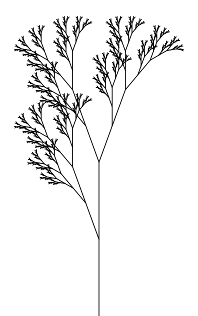
\includegraphics[scale=0.35]{./chapter2/fig/plant.png}
\caption{Graphical representation}\label{fig:plant}
\end{subfigure}
\hspace{2.6cm}
\begin{subfigure} {\linewidth}\centering
\begin{lstlisting}[language=java, basicstyle=\footnotesize, stringstyle=\footnotesize\color{green!70!black}]
String P0 = "FF[+F[+X]F[-X]+X]FF[-F[+X]F[-X]+X]+F[+X]F[-X]+X";
\end{lstlisting}
\caption{Java code generated after translation (two iterations instead of seven)}\label{fig:l-system-generated}
\end{subfigure}
\end{mdframed}
\caption{Simple OL-System to generate a plant in two dimensions. On the left} \label{lst:OL-system-example}
\end{figure}

Apart from the characteristics of each DSL, an important \textbf{feature to consider by engineers who implement support for resource awareness} for a DSL,
is that languages do not always provide well-defined boundaries as software components do.
For instance, an internal DSL may be transformed into a list of statements of the host language without defining a new routine or thread.
In a case like this, instrumentation is the only mechanism that can be used to achieve CPU consumption monitoring.

Interestingly, interaction between programs written using DSLs can also impact the way resource accounting is done.
In the state machine example previously discussed, a state machine might trigger events in another state machine by simple executing some actions in one of its transitions.
This is closely related to the problem of accounting resource consumption in components that are interacting.

The \textit{state machine} and \textit{L-system} languages clearly reflect \textbf{differences between DSLs}.
These differences are not surprising.
Languages consume resources in different ways; some languages only consume memory while others consume CPU or other resources.
The capacity to monitor the consumption of a program written using a DSL is related to factors such as,
the specific meaning of the involved concepts,
and the translational semantic of the language.

\paragraph{State of the art on providing resource awareness support for DSLs}
As far as we know, there is little support for dealing with resource at per DSL level.
Nevertheless, some related works do exist that aim at reducing the gap between the developer's view and the tools' view.
In particular, the problem of offering debugging support for DSL constructs have been largely discussed.
In Xtext~\cite{Eysholdt:2010:XIY:1869542.1869625}, languages that produce code in the base language (i.e., Java) may profit from mostly automatic debugger support.
When the newly define DSL is transformed into the base language, the system keeps traces between the two models (source and destination).
Using these traces, a debugging infrastructure is able to identify what constructor is being executed in the original DSL.
Meanwhile, Voelter \cite{Voelter2010} discusses how to add debugging capabilities to a DSL when the MPS language workbench is used.
In this case, no trace model is required; instead, every concept of a language that requires debugging support must implement a set of interfaces to guide a generic debugging framework.
Similar works have been conducted \cite{vandenBrand:2005:TGD:1705513.1705667} for the ASF+SDF Meta-Environment \cite{vandenBrand20013}, defining a generic debugging framework that can be customized for DSLs.
Finally, mechanisms to build various tools for new languages are described in \cite{Henriques2005}.
Based on attribute grammars, and implemented using the LISA system \cite{Mernik2002}; the tools proposed include editors, inspectors, debuggers and visualizers.

%\extracomment{TODO}{Add discussion on how to ad plugins for Eclipse MAT and VisualVM}

%Profilers: visualvm
%
%low-Level profiling technologies: JVMTI, DTrace
%
%In~\cite{Xu:2013:PML:2491509.2491511} the authors propose a framework to detect memory leaks associated with Java containers.
%To do so, the framework explores the status of each container object with the goal of identifying leak patterns.
%
%LeakBots~\cite{Mitchell03leakbot:an} is an automated tool to detect memory leaks. It makes heavy
%use of information collected from the heap in order to identify the more likely structures leading to a leak.
%These tools collect data from the heap in order to automatically pinpoint a particular memory issue.
%The methods to collect the data are handwritten for efficiency reasons.
%Lots of data collected in these works is also available with our approach.

\subsection{Limitations of the state of the art on dealing with abstraction-specific features}

In reviewing the state of the art, we have found some limitations on how existent solutions deal with specific features of abstractions.
In this section we discuss such limitations:


\begin{description}

\item[Limited support for resource accounting in component-based systems] There are several approaches for monitoring how individual components use resources.
However, they are limited and inefficient.
First, most of them only target mainstream component models such as OSGi and EJB; this is a fact noteworthy because it is not clear whether the ideas behind existent approaches can be applied to other component models.
The second and more important problem is the considerable overhead induced by these solutions.
In the case of memory consumption accounting, the best results we found show a persistent overhead of 46\% (medium).
By comparison, experiments of CPU consumption accounting show a lower overhead of 20\% when \textit{sampling} is used.
In many scenarios, these overheads are unacceptable. 

\item[Sub-utilization of information about the architecture of systems].
Actually, all approaches use rudimentary information about the architecture of the system running on top a component framework.
In other words, they are able to determine how each component consume resources (regardless of the accuracy).
As shown in \cite{Maurel:2012:AME:2304736.2304763}, it is possible to use information on how components are connected (their dependencies) to improve the monitoring accuracy.
Similarly, Attouchi et al. \cite{Attouchi:2014:MMM:2602458.2602467} show how to use the knowledge about the \textit{business logic} (in particular how components interact) to properly determine what component should be accounted for the consumption of an object.
Nevertheless, we have not found results showing how to reduce performance overhead by using information about the architecture of component-based systems. 


\item[Non-portable solution for resource isolation] Existent approaches to provide per-component resource consumption isolation require a modified MRTE.
In practice, this prevents the adoption of these approaches in production environments; due to the cost of maintaining a customized MRTE, and the complexity of keeping it up to date, manager  with a limited budget can decide that these solutions are not acceptable.

%\item Only widely used component models such as OSGi, and EJB, have support for resource management.

\item[Wrongly assume that resource consumption is homogeneous]
Although components use computational resources in different ways, many approaches to resource consumption and reservation are built without taking this into consideration.
A negative consequence of this limitation is that they induce a high overhead even if the components are behaving in the proper way.
For instance, some monitoring frameworks to calculate CPU consumption induce a persistent overhead; it does not matter that components never misbehave.
Instead, adaptive mechanisms are preferable because they have the potential of reducing the overhead by analyzing the requirements and observing the status of the system.
%Las soluciones son handcrafted y staticas, no se adaptan a lo que los componentes necesitan realmente (contrario a Squirrel)\

\item[Limited capabilities for building tooling support] Debuggers, interpreters and simulator have been proposed as tools to support the maintenance of software written using DSLs; however, as far as we know, no profiler that specifically aims at reducing the gap between DSLs and base language have been presented.
It is worth mentioning that some general profiling frameworks can be used to ease the construction of profilers, even if they do not specifically address DSLs; these mechanisms as well as their limitations are discussed hereafter.

\end{description}



\section{Easing the construction of resource management tools} \label{sec:easy-tools-contruction}

Resource consumption monitoring is a form of dynamic analysis.
There are many approaches that tackle the issue of simplifying the definition of dynamic analysis tools.
On the contrary, we have found fewer mechanisms to ease the construction of resource reservation tools \cite{mueller}.
Due to this fact, we mostly discuss the problem of supporting resource accounting. 

The next section presents a variety of approaches. The following properties are discussed for each approach:

\begin{description}
\item[Generality] Indicate the expressive power of the approach. We only consider two values: \textit{arbitrary} and \textit{limited}.

\item[Ease of use] We argue that the possible values are \textit{already known language}, \textit{new DSL}, \textit{require specific knowledge of the MRTE}.

\item[Performance Overhead] As in the previous paragraph we use the values \textit{low}, \textit{medium}, and \textit{high}.
Likewise, these values are taken from the literature review.
\end{description}

\subsection{Flexible implementation of dynamic analysis tools}

One of the most tedious and error-prone tasks, when building tooling support for dynamic analysis, is dealing with low-level details such as, bytecode instrumentation.
If dynamic analysis tools are built from the scratch, developers are forced to focus on mastering details of the execution platform, when in fact, they are interested in implementing high-level ideas.
To address this issue, various approaches have been proposed; they can be clustered into three categories: instrumentation frameworks, high-level APIs for bytecode manipulation, and aspect-oriented tools.

Several instrumentation frameworks for MRTEs have been proposed.
In \cite{Liang1999}, the authors propose the JVM Profiling Interface (JVMPI); a set of low-level facilities built-in the JVM to trigger notifications when certain events occur during application execution.
Although the events reported only provide primitive information, such as \textit{method invoked} and \textit{thread created}, this basic data can be used along other infrastructure to build more powerful tools.
Severe limitations prevented the success of JVMPI (deprecated in favor of JVMTI): performance impact on the JVM, the relatively low-level interface provided, and the limited capabilities to detect fine-grained events.
These limitations are partially addressed in \cite{Maebe06javana:a} where a framework called Javana is proposed.
In specific, Javana proposes further modifications to the JVM to detect more events.
Additionally, it aims at easing the construction of efficient user-defined profilers by providing a generic instrumentation framework which can be adapted to specific needs.
To do so, users define a profile using an aspect-inspired DSL where \textit{pointcuts} represent the events of interest for a profilers, and advices, which are written in \textit{C/C++}, are in charge of collecting data on the dynamic behavior of a program.
Besides the problem of requiring a modified JVM, this approach also has other disadvantages such as demanding a deep understanding of the JVM.
A profiling framework that instruments Java programs at the bytecode level to build context-sensitive execution profiles at runtime is proposed in \cite{Binder2005}.
The profiling framework includes an exact profiler as well as a sampling profiler.
Users can define their own profilers using a provided infrastructure for program transformation.
The most interesting point is that profilers are written in pure Java; this can low the barrier for Java developers who devise customized profiling strategies.
Finally, Reiss proposes \cite{Reiss:2008:CDP:1383559.1383566} a framework, DYPER, to organize and schedule the execution of monitoring agents.
Each agent (so-called proflet) is able to obtain data, regarding some properties, using two approaches.
Through sampling the data collected have poor quality, while data collected using instrumentation are very detailed.
The framework schedules the execution of proflets to guarantee a bound on monitoring overhead.
To perform the scheduling, each proflet provides an estimates of both the expected application overhead and the time needed to set up the detailed monitoring; this information is used to dispatch the execution of a detailed collection of data.
In practice, this is a form of adaptive monitoring where mechanisms with high overhead are executed only when possible.
Proflets are built using either Java or C, and they can be composed in order to collect more complex data.
The main limitation of this approach, beside from the fact that no experimental validation is provided, lies on the difficulty of properly estimating the overhead of proflets.

The usage of bytecode instrumentation techniques to build dynamic analysis tools have leaded to the development of high-level APIs for bytecode rewriting.
For instance, ASM~\cite{Bruneton2002,Kuleshov2007} is a Java bytecode manipulation and analysis framework written itself in Java.
It is useful to transform classes directly in binary form.
To do so, it provides common transformations and analysis algorithms to assemble custom transformations.
Alas, it requires considerable knowledge regarding the JVM specification.
In particular, it is mandatory to understand the Java instruction set, how are they executed, and the basic structure of a classfile in Java.
By comparison, Javassist \cite{Javassist1999} simplifies Java bytecode manipulation.
It is a class library for editing bytecodes in Java; however, unlike ASM, it provides a source level API: to transform a classfile without knowledge of the specifications of the Java bytecode.
For example, you can specify what bytecode to insert in an existent class by using plain Java source code - Javassist compiles it on the fly and inserts it on the class being transformed.

The collection of data for a given dynamic analysis can be easily understood as a crosscutting concern.
Because of this, researchers have been attracted by aspect-oriented solutions.
Indeed, aspect-oriented frameworks already provide the mechanisms to i) specify multiple points of interest in the binary code of an application, and ii) execute handlers when the program counter reaches these locations.
In other words, by simply defining aspects (\textit{pointcuts} and \textit{advices}), developers can focus on the high-level ideas of dynamic analysis.
Nonetheless, aspect-oriented solutions are not flawless; some limitations have prevented its adoption in this field.
An interesting evaluation of the positive and negatives points of using aspect-oriented dynamic analysis is presented in \cite{Pearce:2007:PA:1248445.1248448}.
In addition to four dynamic analysis presented and evaluated (showing medium or high overhead), the authors also discuss how the \textit{pointcuts} of AspectJ are not sufficient to achieve better performance and to create more analysis.
The issue of improving the performance is tackled by Binder et al. \cite{Binder:2006:FEM:1173706.1173733}.
In their work, the MAJOR~\cite{Villazon20111015} framework, an aspect weaver that enhances AspectJ with support for comprehensive weaving, is extended to guarantee fast sharing of values between aspects.
This simple addition is enough to reduce the performance overhead of some dynamic analysis.
DISL~\cite{Marek:2012:DEL:2162037.2162046,Marek2012} is a domain-specific aspect language for bytecode instrumentation; it uses annotations and plain Java to describe what a dynamic analysis tool must do.
The novelty of this approach is that new \textit{joinpoints} and \textit{guard conditions} can be defined using the Java language along some annotations.
It is then possible to collect data which is not accessible using a standard framework such as AspectJ.
Unfortunately, to define new \textit{jointpoints}, some knowledge of JVM internals is required.
Finally, in an effort to overcome the limitations of specific aspect weavers, which prevent using them to implement arbitrary dynamic analysis tools, Achenbach et al.~\cite{Achenbach:2010:MPD:1939399.1939415} propose an approach to customize aspect weavers.
When a new concrete weaver is built, the developer can choose arbitrary locations in the program as \textit{joinpoints}.
In the same way, different strategies to weave \textit{advices} can be implemented.
Implemented in Ruby, the approach is evaluated through the definition of a debugger and a testing tool.

Other approaches focus on profiling the memory usage of applications.
Memory profilers that are widely used in the industry provide languages to perform mostly arbitrary queries on the set of objects loaded in the heap.
For instance, in Eclipse MAT \cite{Biermann:2006:GDI:2087202.2087244} and Visual VM \cite{OQL-visualvm}, users can write queries in OQL (a SQL-like language) to retrieve information.
Despite of the fact that few constructors of OQL are really implemented in Eclipse MAT, this approach would allow, in theory, collecting practically any information contained in the heap.
Similarly, YourKit \cite{yourkit} provides a language based on set theory to filter objects with specific properties; this language is used when no built-in memory analysis can provide the desired data.
Besides providing query languages, mainstream profilers also support the development of extensions (e.i., plugins written in Java); these extensions essentially traverse the graph of objects in a heap dump to collect information.
Alas, both queries and extensions require costly operations - a complete dump of the heap, and a phase to preprocess the dump; only after these operations, the frameworks are capable of executing queries.
In DeAl~\cite{Reichenbach:2010:GCE:1869459.1869482}, the authors propose a language to compute heap assertions at garbage collection time.
The design of this approach aims at guarantee a low performance overhead.
To ensure such a property, the language is only able to compute boolean outputs; while resource consumption monitoring, for instance, needs to compute values of integer type.
DeAl is a purely declarative language; in exchange for the declarative style and the focus on assertions, some formal properties apply to DeAl. 

\subsection{Discussing the limitations}

Although there exists many approaches that aim at reducing the complexity of writing tools to support resource-aware programming, in reviewing the literature we have found some limitations that prevent using such solutions in production environments.
In particular, the identified limitations are related to three dimensions we can use to assess the overall quality of a mechanism: many techniques still require considerable knowledge about the target technology, tools built using existent approaches often induce high performance overhead, and most solutions lack the power to express how to build efficient tools.
Unsurprisingly, these three dimensions are often in contradictions.
For instance, most approaches that offer good performance overhead require considerable knowledge about the target technology.
The question is whether the trade-offs followed by different approaches are good enough.
In this section, we discuss in details the limitations we find in the state of the art.

\begin{description}
\item[Tools built using the approaches have high overhead]
Many times, the tools that we can build using the approaches presented in the previous section induce high overhead.
This is particularly true for solutions based on bytecode rewriting, but also for other approaches, such as JVMPI, that are based on events.
This is not surprising; as we discuss in the previous chapter, bytecode rewriting and other techniques tend to produce high overhead.
The mechanisms that are able to keep a low overhead, do so by limiting the expressive power of the tools (as in DeAl~\cite{Reichenbach:2010:GCE:1869459.1869482}), and by reducing the accuracy of the tools in certain cases (as in DYPER \cite{Reiss:2008:CDP:1383559.1383566}). 


\item[Often, knowledge of low-level details is required] 
The usability of a mechanism is complex to evaluate; the approaches we have presented have not been assessed in this dimension.
Instead, these approaches follow empirical evidence that show the benefits of specific techniques.
One of this evidences suggests that using already known languages may ease the development of dynamic analysis tools.
Hence, some solutions encourage the usage of Java to build profilers and others the utilization of a SQL-like language.
Likewise, the empirical evidence suggests that paradigms, such as aspect-oriented programming, and functional programming, should be favored.
The problem is that using known-languages and programming paradigms do not automatically reduce the complexity of writing tools.
Actually, often the complexity is the result of having to deal with low-level details about the platform,
and many techniques still require considerable knowledge of the target platform.
In the same way, using aspect-oriented programming can also create additional problems.
Indeed, since well-known frameworks, such as AspectJ, cannot be used to develop any profiler, new and unknown aspect frameworks must be used to implement such profilers.

We think that approaches that use languages such as \textit{C/C++} may also complicate the developments of tools.
Unfortunately, many techniques with low overhead can eb implemented using low-level technologies (such as JVMTI), or through a modification to a legacy MRTE.

\item[Lack of expressive power to build efficient tools] 
Powerful tools can be indeed produced using existent approaches.
It does not mean that they are efficient.
The problem is that, when a solution is expressive and produce efficient tools, it generally require extensive knowledge about low-level details.
Similarly, there is another interesting trade-off we have found; efficient tools that do not require detailed knowledge about the platform, have limited power to create arbitrary tools. 
\end{description}

\extracomment{FIXME :-)}{I must finish this}

%\paragraph{DiSL: a domain-specific language for bytecode instrumentation, \cite{Marek:2012:DEL:2162037.2162046,Marek2012}}
%Dynamic program analysis tools support numerous software engineering tasks, including profiling, debugging, and re-
%verse engineering.
%Prevailing techniques for building dynamic analysis tools are based on low-level abstractions
%that make tool development tedious, error-prone, and expensive. To simplify the development of dynamic analysis tools,
%some researchers promoted the use of aspect-oriented programming (AOP). However, as mainstream AOP languages
%have not been designed to meet the requirements of dynamic analysis, the success of using AOP in this context remains
%limited. For example, in AspectJ, join points that are important for dynamic program analysis (e.g., the execution of
%bytecodes or basic blocks of code) are missing, access to reflective dynamic join point information is expensive, data
%passing between woven advice in local variables is not supported, and the mixing of low-level bytecode instrumentation
%and high-level AOP code is not foreseen. In this talk, we present DiSL [1], a new domain-specific aspect language for
%bytecode instrumentation.
%DiSL uses Java annotation syntax such that standard Java compilers can be used for compiling
%DiSL code. The language features an open join point model, novel constructs inspired by weave-time evaluation of
%conditional join points and by staged execution, and access to custom static and dynamic context information.
%Moreover, the DiSL weaver guarantees complete bytecode coverage.
%We have implemented several dynamic analysis tools in DiSL,
%including profilers for the inter- and intra-procedural control
%flow, debuggers, dynamic metrics collectors integrated in the
%Eclipse IDE to augment the static source views with dynamic information, and tools for workload characterization.
%These tools are concise and perform equally well as implementations using low-level techniques. DiSL has also been
%conceived as an intermediate language for future domain-specific analysis languages, as well as for AOP languages.
%
%\paragraph{Javana: A System for Building Customized Java Program Analysis Tools, \cite{Maebe06javana:a}}
%Understanding the behavior of applications running on high-level
%language virtual machines, as is the case in Java, is non-trivial because of the tight entanglement at the lowest execution level between the application and the virtual machine.
%
%This paper proposes Javana, a system for building Java program analysis tools.
%Javana provides an easy-to-use instrumentation infrastructure that allows
%for building customized profiling tools very quickly.
%Javana runs a dynamic binary instrumentation tool underneath
%the virtual machine. The virtual machine communicates with the
%instrumentation layer through an event handling mechanism for
%building a vertical map that links low-level native instruction pointers and memory addresses to high-level language concepts such as
%objects, methods, threads, lines of code, etc.
%The dynamic binary instrumentation tool then intercepts all memory accesses and instructions executed and provides the Javana end user with high-
%level language information for all memory accesses and natively
%executed instructions.
%
%We demonstrate the power of Javana through a number of applications: memory address tracing, vertical cache simulation and
%object lifetime computation.
%For each of these applications, the instrumentation specification requires only a small number of lines
%of code.
%Developing similarly powerful profiling tools within a virtual machine (as done in current practice) is both time-consuming
%and error-prone; in addition, the accuracy of the obtained profiling
%results might be questionable as we show in this paper.
%\paragraph{Flexible and efficient profiling with aspect-oriented programming, \cite{Binder:2006:FEM:1173706.1173733}}
%Many profilers for virtual execution environments, such as the Java virtual machine (JVM), are implemented with low-level bytecode instrumentation techniques, which is tedious, error-prone, and complicates maintenance and extension of the tools.
%In order to reduce the development time and cost, we promote building profilers for the JVM using high-level aspect-oriented programming (AOP).
%We show that the use of aspects yields concise profilers that are easy to develop, extend, and maintain, because low-level
%instrumentation details are hidden from the tool developer.
%In order to build efficient profilers, we introduce inter-advice communication, an extension to common AOP languages that enables efficient data passing
%between advices that are woven into the same method using local variables.
%We illustrate our approach with two case studies.
%First, we show that an existing, instrumentation-based tool for listener latency
%profiling can be easily recast as an aspect.
%Second, we present an aspect for comprehensive calling context profiling.
%In order to reduce profiling overhead, our aspect parallelizes application execution and profile
%creation, resulting in a speedup of 110\% on a machine with more than two cores, compared with a primitive, non-parallel approach
%\paragraph{A portable and customizable profiling framework for Java based on bytecode instruction counting, \cite{Binder2005}}
%Prevailing profilers for Java, which rely on standard, native-code profiling interfaces, are not portable, give imprecise results due to serious measurement perturbation, and cause excessive overheads.
%In contrast, program transformations allow to generate reproducible profiles in a fully portable way with significantly less overhead.
%This paper presents a profiling framework that instruments Java programs at the bytecode level to build context-sensitive execution profiles at runtime.
%The profiling framework includes an exact profiler as well as a sampling profiler.
%User-defined profiling agents can be written in pure Java, too, in order to customize the runtime processing of profiling data.
%\paragraph{Profiling with AspectJ, \cite{Pearce:2007:PA:1248445.1248448}}
%This paper investigates whether AspectJ can be used for efficient profiling of Java programs.
%Profiling differs from other applications of AOP (e.g. tracing), since it necessitates efficient and often complex
%interactions with the target program.
%As such, it was uncertain whether AspectJ could achieve this goal.
%Therefore, we investigate four common profiling problems (heap usage, object lifetime, wasted time and
%time-spent) and report on how well AspectJ handles them.
%For each, we provide an efficient implementation,
%discuss any trade-offs or limitations and present the results of an experimental evaluation into the costs
%of using it.
%Our conclusions are mixed. On the one hand, we find that AspectJ is sufficiently expressive
%to describe the four profiling problems and reasonably efficient in most cases.
%On the other hand, we find several limitations with the current AspectJ implementation that severely hamper its suitability for
%profiling.
%
%\paragraph{Controlled dynamic performance analysis, \cite{Reiss:2008:CDP:1383559.1383566}}
%We are interested in obtaining detailed performance information
%on-the-fly from long-running systems without adversely affecting
%the performance of the systems.
%We have developed a methodology consisting of a framework, DYPER, and a number of
%specialized agents called proflets each of which analyzes a
%different performance aspect.
%DYPER gathers performance information with a guaranteed maximum overhead that is
%dynamically settable by the programmer using priorities set by the
%proflets.
%Moreover, the type of information that the system can
%provide is generally only available for tools that generally have too
%much overhead to be usable in production or long-running
%systems.
%DYPER includes the ability to control and display
%performance data as the program is run.
%
%\paragraph{A meta-aspect protocol for developing dynamic analyses, \cite{Achenbach:2010:MPD:1939399.1939415} }
%Dynamic aspect-oriented programming has been widely used
%for the development of dynamic analyses to abstract over low-level program instrumentation.
%Due to particular feature requirements in different analysis domains like debugging or testing, many different aspect
%languages were developed from scratch or by extensive compiler or interpreter extensions.
%We introduce another level of abstraction in form of a meta-aspect protocol to separate the host language from the analysis
%domain.
%A language expert can use this protocol to tailor an analysis-specific aspect language, based on which a domain expert can develop
%a particular analysis.
%Our design enables a flexible specification of the join point model, configurability of aspect deployment and scoping, and
%extensibility of pointcut and advice language.
%We present the application of our design to different dynamic analysis domains.
%
%\paragraph{Comprehensive Profiling Support in the Java Virtual Machine. \cite{Liang1999}}
%Existing profilers for Java applications typically rely on custom instrumentation in the Java virtual machine, and measure only limited types of resource consumption. Garbage collection and multi-threading pose additional challenges to profiler design and implementation.
%
%In this paper we discuss a general-purpose, portable, and extensible approach for obtaining comprehensive profiling information from the Java virtual machine. Profilers based on this framework can uncover CPU usage hot spots, heavy memory allocation sites, unnecessary object retention, contended monitors, and thread deadlocks. In addition, we discuss a novel algorithm for thread-aware statistical CPU time profiling, a heap profiling technique independent of the garbage collection implementation, and support for interactive profiling with minimum overhead.
 
%\paragraph{Profiling Field Initialisation in Java, \cite{Nelson2013}}
%\todo{No cre que sea muy bueno}
%Java encourages programmers to use constructor methods to
%initialise objects, supports final modifiers for documenting fields which
%are never modified and employs static checking to ensure such fields
%are only ever initialised inside constructors. Unkel and Lam observed
%that relatively few fields are actually declared final and showed using
%static analysis that many more fields have final behaviour, and even more
%fields are stationary (i.e. all writes occur before all reads). We present
%results from a runtime analysis of 14 real-world Java programs which
%not only replicates Unkel and Lam’s results, but suggests their analysis
%may have under-approximated the true figure. Our results indicate a
%remarkable 72-82% of fields are stationary, that final is poorly utilised by
%Java programmers, and that initialisation of immutable fields frequently
%occurs after constructor return. This suggests that the final modifier for
%fields does a poor job of supporting common programming practices.
%\paragraph{A dynamic optimization framework for a Java just-in-time compiler, \cite{Suganuma:2001:DOF:504311.504296}}
%The high performance implementation of Java Virtual Machines (JVM) and just-in-time (JIT) compilers is directed toward adaptive compilation optimizations on the basis of online runtime profile information. This paper describes the design and implementation of a dynamic optimization framework in a production-level Java JIT compiler. Our approach is to employ a mixed mode interpreter and a three level optimizing compiler, supporting quick, full, and special optimization, each of which has a different set of tradeoffs between compilation overhead and execution speed. a lightweight sampling profiler operates continuously during the entire program's exectuion. When necessary, detailed information on runtime behavior is collected by dynmiacally generating instrumentation code which can be installed to and uninstalled from the specified recompilation target code. Value profiling with this instrumentation mechanism allows fully automatic code specialization to be performed on the basis of specific parameter values or global data at the highest optimization level. The experimental results show that our approach offers high performance and a low code expansion ratio in both program startup and steady state measurements in comparison to the compile-only approach, and that the code specialization can also contribute modest performance improvement.
%
%\paragraph{Complete and Platform-Independent Calling Context Profiling for the Java Virtual Machine, \cite{Sarimbekov201161}}
%Calling context profiling collects statistics separately for each calling context. Complete calling context profiles that faithfully represent overall program execution are important for a sound analysis of program behavior, which in turn is important for program understanding, reverse engineering, and workload characterization. Many existing calling context profilers for Java rely on sampling or on incomplete instrumentation techniques, yielding incomplete profiles; others rely on Java Virtual Machine (JVM) modifications or work only with one specific JVM, thus compromising portability. In this paper we present a new calling context profiler for Java that reconciles completeness of the collected profiles and full compatibility with any standard JVM. In order to reduce measurement perturbation, our profiler collects platform-independent dynamic metrics, such as the number of method invocations and the number of executed bytecodes. In contrast to prevailing calling context profilers, our tool is able to distinguish between multiple call sites in a method and supports selective profiling of (the dynamic extent of) certain methods. We have evaluate the overhead introduced by our profiler with standard Java and Scala benchmarks on a range of different JVMs.


%\paragraph{another, \cite{Harkema:2002:PMJ:584369.584388}}



\begin{comment}

\section{Resource Awareness for Domain-specific Abstractions} \label{sec:resource-awareness-for-dsl}


\subsection{Debugging support for DSLs}

\end{comment}

\section{Conclusions}


Defining and using software abstractions is at the core of system development.
Once a new abstraction is defined, the tools used in the development process and to support resource awareness should be modified to make them reflect the new concepts.
When these modification are not done, we argue that a mismatch exists between developer's view and the tooling's view.
However, implementing this tooling support is tedious and error-pone.
In this chapter, we have identified two challenges related to this complexity:

\begin{itemize}
\item A concrete abstraction may have specific features to consider when implementing tooling support.
On the one hand, this features can derive into additional requirements for the tools, making even more complicated their implementation.
On the other hand, some features can be useful to drive the behavior of systems that require support for resource awareness.

\item Given the mainstream trend of defining new software abstractions (for example with DSLs), it is necessary to ease the task of building their support.
For instance, building a resource consumption monitor for a new DSL should simple enough as to make it affordable for DSL developers.
\end{itemize}   

In reviewing the state of the art of resource management for software abstractions, we realized that there are severe shortcomings in existent approaches that prevent their usage in production environments. In particular:

\begin{itemize}
\item Approaches to extract \textit{arbitrary} information from memory (e.g., number of objects of a given class, class of each that object that references an array) are too expensive in terms of performance overhead.

\item Several approaches for defining dynamic analysis tools rely on instrumentation to collect data. 
\end{itemize} 

%
%Discutir aqui que problemas nuevos surgen cuando se quiere hacer resource management en component-based systems. Por ejemplo, a quien se le asigna el consumo.


